% ---- ETD Document Class and Useful Packages ---- %
\documentclass{ucetd}
\usepackage{subfigure,epsfig,amsfonts}
\usepackage{natbib}
\usepackage{amsmath}
\usepackage{amssymb}
\usepackage{amsthm}
\usepackage[toc,page]{appendix}
\usepackage[labelfont=bf]{caption}

\usepackage{url}
 

%% Use these commands to set biographic information for the title page:
\title{Stochastic computation in recurrent networks of spiking neurons}
\author{Clayton W. Seitz}
\department{Graduate Program in Biophysics}
\division{Physical and Biological Sciences}
\degree{Master of Science}
\date{Winter 2021}

%% Use these commands to set a dedication and epigraph text

\epigraph{Epigraph}

\begin{document}
%% Basic setup commands
% If you don't want a title page comment out the next line and uncomment the line after it:
\maketitle
%\omittitle

% These lines can be commented out to disable the copyright/dedication/epigraph pages
\makecopyright
%\makededication
\makeepigraph


%% Make the various tables of contents
\tableofcontents
%\listoffigures
%\listoftables

\acknowledgments
% Enter Acknowledgements here

\abstract

The primate cerebral cortex is a complex system estimated to harbor more than 25 billion neurons communicating via action potentials or `spikes' and is responsible for many higher-order brain functions including memory and learning. Recent years have hosted many efforts to understand how such complex phenomena emerge from the communication of individual cells. Many studies have provided evidence that long term plasticity (LTP) in synapses permits a long-lasting alteration of network dynamics and, in turn, forms the basis of long-term memory and learning. However, understanding memory formation and learning in the brain is made difficult by the variability in the response of cortical neurons to stimuli. Therefore, capturing the apparent stochastic features of neural activity in computer based models, such as recurrent spiking neural networks (RSNNs), while explaining their manipulation of information mathematically has become the gold standard for computational neuroscience. Models of neural networks derived from statistical mechanics, such as those which assert that the membrane potential of a cortical neuron obeys a form of Langevin dynamics, can potentially account for stochastic network activity. Such models also provide the intriguing interpretation that neural activity represents sampling from a probability distribution - a technique central to statistical inference.  Here, we apply a similiar mathematical treatment to the study of an RSNN by modeling the membrane potential statistics of an integrate and fire neuron using Fokker-Planck equations. With this statistical framework in hand, we can recast a network of neurons as a stochastic process in higher dimensions and explore the relationships between synaptic connectivity and its plasticity to the correlation structure of neural spike trains. This approach is also amenable to information theoretic analysis and is a step toward a mathematical relationship between neuroplasticity mechanisms and the emergent computational capabilities of cortical microcircuits.



\mainmatter

\chapter{Models of action potential generation}

The dominating information processing unit in neocortex is the spiking neuron - a neural cell which exhibits transient depolarization of the cell membrane called action potentials or\emph{spikes}. The potential is regulated by a diverse set of highly specific ion channels embedded in the plasma membrane which open and close based on environmental factors such as the membrane potential itself or changes in the concentration of neurotransmitters. This dependence of the so-called \emph{open probability} of ion channels results in changes of the membrane conductance for the ions they transport and is the origin of the non-linear properties of  cells in the nervous system. Several mathematical models have been proposed to explain this process in various levels of detail, generally depending on their application. Some consider the biophysical details of action potential generation by considering specific types of ion channels and their dynamics while others neglect such details for the sake of mathematical simplicity. At the same time, models are often classified as conductance-based or current-based, depending on whether they model the membrane conductance explicitly or summarize membrane depolarization as a sum of membrane currents. The famous Hodgkin-Huxley (HH) model published in 1952 was originally used to fit experimental voltage traces measured in the squid giant axon and is arguably the most biophysically accurate of model of membrane depolarization. The membrane potential of an HH neuron evolves according to a a set of ordinary differential equations that include a term for each of the ion channels thought to be critical for the generation of an action potential. In the following paragraphs, we will briefly introduce the Hodgkin-Huxley model alongside an integrate and fire (IF) model to provide context for the following chapters.

\section{A Brief Overview of Neuron Models}

The integrate and fire (IF) model of a cortical neuron has become a standard tool for exploring neuronal dynamics. It's relative simplicity makes it an appealing choice for large scale simulations where the precise details of synaptic transmission can be neglected and a neuron can be described with only a few state variables. A large body of research has shown that precise timing of action potentials has an important role in neural information processing - a feature central to the IF model (Rieke, 1997). However, it is important to note that the IF model remains a coarse approximation to the diverse set of neurons observed thus far in cortex. Biophysical models such as the Hodgkin-Huxley model are known to describe action potential generation more precisely than IF models, but have the significant drawback that they are computationally expensive. Even the minimalist IF model presents substantial barriers to theoretical analysis (Brunel 2000). On the other hand, IF models have been shown to capture a diverse set of dynamical states observed in cortex (Citation). 

Noisy variants of IF models have been introduced to summarize the enormous number of degrees of freedom due to millions of ion channels and thousands of presynaptic signals impinging on the neuron (Tuckwell 1989, Plesser 2000). Such models describe the inputs to a neuron by decomposing the total synaptic input into a deterministic part $I(t)$ and a stochastic part $\xi(t)$, which is taken to be a gaussian white noise (GWN). 

\begin{align}
\tau\dot{V_{j}} = -V_{j} + \mu_{j}(t) + \xi_{j}(t)
\end{align}

The variables $\mu(t)$ and $\xi(t)$ are interpreted as post-synaptic potentials (PSPs) and thus have dimensions of voltage. Eq. (1.1) has the form of a well-known stochastic differential equation (SDE) called the Langevin equation. When the voltage $V$ crosses a firing threshold $\Theta$, we say the neuron has fired an action potential and the voltage is reset to the resting value $V_{R}$. Therefore, we define an additional state variable $z(t) = H(V-v_{th})$ where $H$ denotes the Heaviside step function.


Stochasticity in IF neurons can be obtained through several mechanisms, such as a noisy reset potential, noisy firing threshold, or intrinsic noise originating in the stochastic features of membrane channels (Plesser and Gerstner 2000, Neftci 2014) or the exocytosis of synaptic vesicles. At the same time, stochastic spike arrival may contribute to fast fluctuations in the membrane potential that cannot be described by a deterministic component $I(t)$. Contrary to intuition, many have suggested that this randomness could contribute positively to the computational paradigm employed in cortical circuits. This phenomenon, referred to as \emph{stochastic resonance} is a property of a dynamical system subject to both periodic forcing and random perturbation may show a resonance only when both the periodic forcing and random perturbation are present (Benzi, 1981). In the context of IF models, the deterministic current $I(t)$ (the summation of post-synaptic potentials) may be subthreshold and $\xi(t)$ is required to push the membrane potential over threshold. Neurons in this regime have a large coefficient of variation just as cortical neurons (Konig, Engel, Singer 1996). More recently, additional evidence has been found that an optimal noise level coincides with the critical regime (Rodriguez 2017) a parameterization of the network that optimizes information transmission (Cramer 2020).

\section{The Ornstein-Uhlenbeck Process}

Langevin equations in the form of (1.1) have been studied extensively and their statistical features have been defined rigorously. In this form, they resemble the Ornstein-Uhlenbeck (OU) process, which is often used in statistical physics to describe a diffusing particle undergoing Brownian motion (Wiener process) with friction. In Brownian motion, the displacement of a variable $x$ in a time $dt$ is normally distributed with variance proportional to $\Delta t$ i.e. $V(t+dt) - V(t) \sim N(0, \sigma^{2}dt)$ or equivalently $dV \sim \sigma\sqrt{dt}\eta(t)$. The Ornstein-Uhlenbeck process is commonly written as a Langevin equation with a noise term similar to Brownian motion but with an added frictional term $-V(t)$ and a non-stationary white-noise $\mu(t) + \sigma\sqrt{dt}\eta(t)$ giving


\begin{equation}
\tau\dot{V_{j}}(t) = -V_{j}(t) + \mu_{j}(t) + \sigma_{j}\sqrt{dt}\eta(t)
\end{equation}

with $\eta(t) \sim \mathcal{N}(0,1)$. This is equivalent to (1.1) with $\xi_{j}(t) = \sigma_{j}\sqrt{dt}\eta(t)$. The last two terms in (1.2) are summarized by the total current arriving at the soma of a neuron $I_{j}(t) = \mu_{j}(t) + \sigma_{j}\sqrt{dt}\eta_{j}(t)$. The solution of (1.2) is a probability distribution over the stochastic variable $V_{j}$ as a function of time i.e. $P(V_{j},t)$. 

\section{The Kramers-Moyal Expansion}

In general, the distribution $P_{j}$ at a time $t'$ can be conditionally dependent on its previous states $t < t'$. Here, we will make the assumption that the evolution of $P_{j}(V_{j},t)$ follows a Markov chain meaning that it has the memoryless property. We are then permitted to write the Chapman-Kolmogorov (CK) equation

\begin{equation}
P(V'_{j}, t) = \int T_{j}(V'_{j}, t | V_{j}, t-\tau)P(V_{j}, t-\tau)dV
\end{equation} 

In terms of (1.2), this requires $\langle\eta(t)\eta(t')\rangle = \delta(t-t')$. Starting from the CK equation in (1.3) we can derive the Kramers-Moyal Expansion (KME) 

\begin{align}
\frac{\partial P_{j}}{\partial t} = \sum_{n} \frac{(-1)^{n}}{n!} \left(\frac{\partial}{\partial V_{j}}\right)^{n} M_{n}(V_{j},t,\tau) P(V_{j},t)
\end{align}

where $M_{n}(V,t,\tau)$ denotes the $nth$ order moment of the transition density $T_{j}(V'_{j}, t | V_{j}, t-\tau)$. If we approximate the KME by truncating the summation for $n > 2$ we arrive at the so-called \emph{diffusion approximation} or Fokker-Planck equation

\begin{align}
\frac{\partial P_{j}}{\partial t} &= \frac{\partial}{\partial V_{j}}[\left(V_{j}(t)-\mu_{j}(t)\right) P_{j}(V_{j},t)] + \frac{\sigma_{j}^{2}(t)}{2}\frac{\partial^{2}}{\partial V_{j}^{2}}[P(V_{j},t)]
\end{align}

where the first and second moments have been substituted by their standard symbols $\mu$ and $\sigma^{2}$.

\section{Fokker-Planck Solution for Unbounded Diffusion}

For the unbounded case of the OU process, the solution of (1.5) is known. The transition density $T_{j}(V_{j}',t+\Delta t|V_{j},t)$ has the following analytical form:

\begin{align}
T_{j}(V_{j}',t+\Delta t|V_{j},t) = \sqrt{\frac{1}{\tau\pi\sigma_{j}^{2}(t)(1-\exp\left(-2\Delta t/\tau)\right))}}\exp\left(-\frac{1}{\tau\sigma_{j}^{2}}\frac{(V_{j}'-V_{R}\exp(-\Delta t/\tau))^{2}}{1-\exp\left(-2\Delta t/\tau\right)}\right)
\end{align} 

This is equivalent to the distribution $P_{j}(V_{j},t)$ as can be seen by plugging $T$ into (2.1) and setting the initial condition $P_{j}(V_{j},t) = \delta(V_{j}-V_{R})$.  An important difference in the IF model in (1.1) and the OU process is that the voltage variable $V$ in the IF model is bounded below by $V_{R}$ and above by the threshold $\Theta$. The reset mechanism requires that $V(t+\Delta t) = V(t)(1-z_{j}(t))$ which is a \emph{renewal process} in the language of statistics, making $V = \Theta$ an absorbing barrier. The bounded case is an example of a first passage time (FPT) problem in statistics where the objective is to find the distribution over times it takes the stochastic variable to diffuse over the barrier. In this context, if we know that a neuron spiked at a time $t^{*}$, we cannot predict the timing of the next action potential. Rather, we can only hope to find the interspike-interval (ISI) distribution $\rho(\tau | t^{*})$ which gives the probability that the next spike occurs at a time $t^{*} + \tau$.  


\chapter{A spatial model of cortical connectivity}

\section{Introduction}

Significant effort has been spent in recent years to map the connectivity patterns of networks in cortex and thus variety of models have appeared. Connection patterns have been quantified by calculating a broad range of structural measures, including small-world attributes and motif composition, as well as some global measures of functional connectivity (Sporns 2006). The structural measures defined in this framework have proven quite useful; however, many models are defined without consideration of the fact that cortical networks are embedded in real space. In principle these spatially-dependent connectivity patterns could be hidden in the topology of an arbitrary graph; however, in some cases it is more straightforward to interpret connectivity patterns in the spatial domain. For example, the connectivity in a 2D lattice of LIF neurons with local and global synaptic connections are readily understood in terms of distances in real space (Rosenbaum 2014). At the same time, theoretical models e.g., mean-field theories of network dynamics have relaxed the strong assumption that cortical networks are spatially homogeneous (Brunel 2000). Defining a periodic connectivity kernel for each neuron on a lattice is an attractive model for cortical networks as it allows us to explore the dynamical consequences of translational invariance.



\section{A statistical framework for spatial connectivity}

The following model for generating the backbone for network of neurons rests on the assumption that we can create connectivity solely from pairwise connection probabilities. Let us define a spatial connectivity kernel $\Gamma_{i}(\mathbf{r}_{j})$ with $i,j\in \{n\}_{n=1}^{N}$ which defines the binomial probability that a neuron $i$ synapses onto a different cell $j\neq i$ at spatial coordinate $\mathbf{r}_{j}$. Here, the function $\Gamma_{i}(\mathbf{r})$ is not itself a probability distribution but rather represents one component of a distribution that is defined for each possible pairs $i,j$ for a given $i$. That distribution is completely represented for a pair $i,j$ with knowledge of the kernel $\Gamma_{j}(\mathbf{r}_{i})$ and an additional probability that no synapse occurs $\Gamma_{0}$. The parameter $\Gamma_{0}$ will be referred to as the $\emph{sparsity parameter}$ throughout the remainder of the text. Together, these three binomial probabilities can be renormalized to form a multinomial distribution $\mathbb{P}_{ij}$ at every possible synapse $ij$. A general definition of the multinomial distribution is

\begin{align}
\mathbb{P} = \frac{p_{n}\prod_{m\neq n}(1-p_{m})}{\sum_{n}p_{n}\prod_{m\neq n}(1-p_{m})} = \frac{p_{n}\prod_{m\neq n}(1-p_{m})}{Z}
\end{align}

where $Z$ is a normalization constant. For generating synapses, the probabilities of (3.1) are the probabilities over the possible synaptic states between $i$ and $j$

\begin{equation}
    \mathbb{P} = \left\{\begin{array}{lr}
        p_{ij} = \Gamma_{ij}(1-\Gamma_{ji})(1-\Gamma_{0})\cdot Z^{-1}\\
        p_{ji} = \Gamma_{ji}(1-\Gamma_{ij})(1-\Gamma_{0})\cdot Z^{-1}\\
        p_{0} = \Gamma_{0}(1-\Gamma_{ij})(1-\Gamma_{ji})\cdot Z^{-1}\\
        \end{array}\right\}
\end{equation}
  
\begin{align*}
Z = \Gamma_{ij}(1-\Gamma_{ji})(1-\Gamma_{0}) + \Gamma_{ji}(1-\Gamma_{ij})(1-\Gamma_{0}) + \Gamma_{0}(1-\Gamma_{ij})(1-\Gamma_{ji})
\end{align*}

Sampling from the distribution $\mathbb{P}$ for each of the $N^{2} - N$ possible synapses (excluding autapses), we can generate an asymmetric adjacency matrix $\mathcal{C} \in \mathbb{F}_{2}^{N\times N}$. An element $\mathcal{C}_{ij} = 1$ defines a synapse from $i\rightarrow j$ and $\mathcal{C}_{ji} = 1$ defines a synapse from $j\rightarrow i$.

Defining the generation of network connectivity in this way proves useful upon the realization that the network can be described by binomial statistics, similar to the well-known Erdos-Renyi (ER) random graph. Graph theory provides a rich set of metrics that can be used to discuss the statistical properties of the network defined by $\mathcal{C}$ and in turn the chosen kernel $\Gamma$. Assuming that we can compute the probabilities $p_{ij}, p_{ji}$ and $p_{0}$ for a particular $\Gamma$ and every synapse is generated independently, the mean of the out-degree distribution is

\begin{equation}
\langle N_{ij} \rangle = \sum_{j} \Gamma_{ij}(1-\Gamma_{ji})(1-\Gamma_{0})\cdot Z^{-1}
\end{equation}

where the spatial dependence of the individual kernels is implied. The in-degree distribution is found by simply swapping $i$ and $j$. The variance of the out-degree distribution is then

\begin{align}
\mathrm{Var}(N_{ij}) &= \sum_{j} \langle N_{ij}^{2} \rangle - \langle N_{ij} \rangle ^{2} \\
&= \sum_{j} \langle N_{ij}\rangle - \langle N_{ij} \rangle ^{2} 
\end{align}

from the linearity of variance property. We will analyze the in-degree and out-degree distributions of a graph generated when the connectivity kernel is a symmetric Gaussian extending over two-dimensions. We refer to this case as a \emph{two-dimensional gaussian network}.


\section{The two-dimensional Gaussian network}

Suppose that we have a two-dimensional lattice which contains points separated by a distance $\Delta$ along the axial directions with periodic boundary conditions. The distance between any two points on such a lattice is the following Euclidean distance metric

\begin{align*}
|\Delta\mathbf{r}_{ij}|^{2} = \mathrm{min}(|x_1 - x_2|, n\Delta - |x_1 - x_2|)^2 + \mathrm{min}(|y_1 - y_2|, n\Delta - |y_1 - y_2|)^2
\end{align*}

Now, let the kernel $\Gamma_{ij}$ be the two-dimensional symmetric Gaussian

\begin{align}
\Gamma_{ij}(|\Delta\mathbf{r}_{ij}|) = \gamma\cdot \exp\left(-\frac{1}{2}(\mathbf{r}_{i}-\mathbf{r}_{j})^{T}\mathbf{\Sigma}_{i}(\mathbf{r}_{i}-\mathbf{r}_{j})\right)
\end{align}

where $\mathbf{\Sigma}_{i} = \sigma_{i}^{2}I$ with the two-dimesional identity matrix $I$. The parameter $\sigma_{i}$ can be intepreted as the \emph{reach} of a neuron $i$. Furthermore, for the kernel $\Gamma_{ij}$ to represent a binomial probability at each point of its domain, we must have that


\begin{equation}
\Gamma_{ij}(|\Delta\mathbf{r}_{ij}|)  \leq 1
\end{equation}

Plugging in our definition (3.5) gives the following inequality

\begin{align*}
\gamma\cdot \exp\left(-\frac{\underset{j}{\mathrm{min}}\left(|\Delta\mathbf{r}_{ij}|^{2}\right)}{2\sigma_{i}^{2}} \right) \leq 1
\end{align*}

The largest possible value of the exponential is achieved at $\underset{j}{\mathrm{min}}\left(|\Delta\mathbf{r}_{ij}|^{2}\right) = \Delta$ (a neighboring lattice point). Therefore, $\gamma$ is upper bounded according to $\gamma \leq \exp\left(\frac{\Delta^{2}}{2\sigma_{i}^{2}}\right)$. For the remainder of our analysis we will fix $\gamma = 1$ and focus our attention to the impact of the parameters $\sigma$ and $\Gamma_{0}$ on the statistics of connectivity. 

As can be seen in Fig. (3.1a), when $\Gamma_{ij} = \Gamma_{ji}$ we have that $p_{ij} = p_{ji}$ for all $|\Delta \mathbf{r}_{ij}|$. We formally refer to this case as the \emph{homogeneous gaussian network}. While this is not necessarily a realistic case, it serves as a useful testbed for the graph theoretic concepts to be used in later analyses. 

\clearpage
\begin{figure}[t!]
\centering
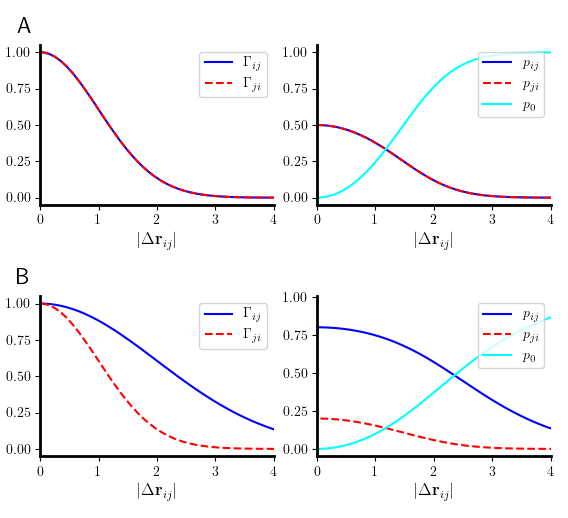
\includegraphics[width=100mm]{fig_11}
\caption{\textbf{Synapse probabilities for gaussian connectivity} (a) Binomial probabilities for two identical gaussian kernels ($\sigma=1$) separated by a distance $|\Delta\mathbf{r}_{ij}|$ and the probability of no synapse $\Gamma_{0}$ (left) and the corresponding multinomial probabilities (right). (b) Binomial probabilities for two different gaussian kernels ($\sigma_{1}=1, \sigma_{2}=2$) separated by a distance $|\Delta\mathbf{r}_{ij}|$ and the probability of no synapse $\Gamma_{0}$ (left) and the corresponding multinomial probabilities (right). }
\end{figure}



\subsection{Homogeneous Gaussian networks}

Let us now examine the statistics of the out-degree of a neuron $i$ assuming that the connectivity parameter $\sigma$ and $\Gamma_{0}$ are homogeneous across the network i.e., they are constant for all neurons. Using Eq. (3.2), we have

\begin{align}
\langle N_{ij} \rangle &= \left(\frac{1-\Gamma_{0}}{N}\right)\sum_{j} \Gamma_{ij}(1-\Gamma_{ji})\cdot Z_{ij}^{-1}
\end{align}

a sum that can be carried out numerically. Interestingly, in the homogeneous case, the parameter $\gamma$ and $\Gamma_{0}$ become redundant. This can be seen by considering that multiplying $p_{ij}$ and $p_{ji}$ by the same constant factor $\gamma$ is equivalent to the transformation $\Gamma_{0}' = 1-\gamma(1-\Gamma_{0})$. 

\clearpage
\begin{figure}[t!]
\centering
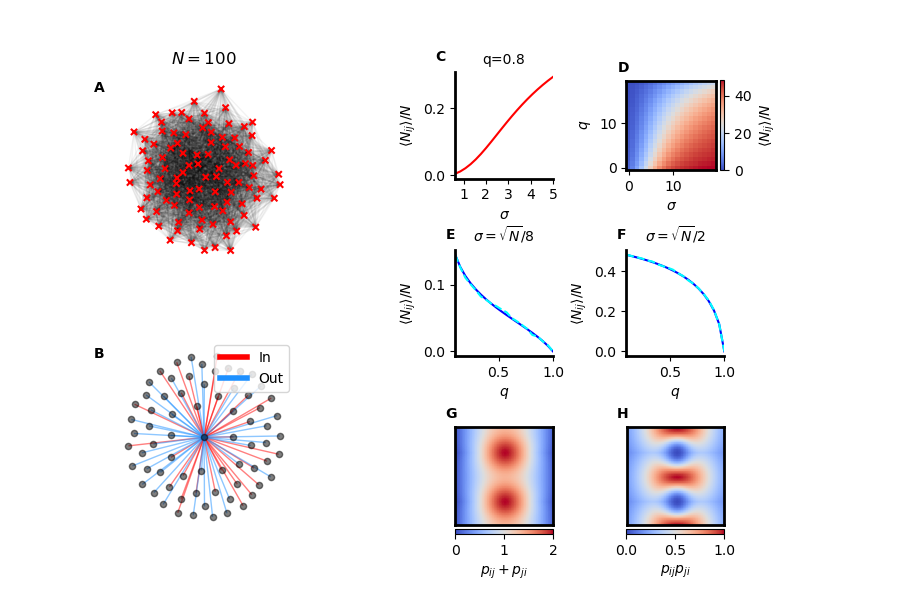
\includegraphics[width=175mm]{fig_8}
\caption{\textbf{The homogeneous Gaussian network}. (A) An example homogeneous network containing $N=100$ neurons. (B) An example neuron extracted from (A) with outgoing synapses labeled in blue and incoming synapses labeled in red. (C,D) The ratio $\langle N_{ij}\rangle/N$ as a function parameters ($\sigma, \Gamma_{0}$) for a sparse network (C) and a network with variable sparsity (D). (E,F) The ratio $\langle N_{ij}\rangle/N$ for fixed $\sigma$ and variable sparsity. (G,H) Binomial probability maps for two nearby neurons expressed as a sum $p_{ij}+p_{ji}$ and product $p_{ij}p_{ji}$}
\end{figure}

In other words, for the homogeneous case, the multiplication by $\gamma$ can be represented by a suitable selection of $\Gamma_{0}$ and can be set $\gamma=1$. Numerical evaluation of (3.7) shows that the ratio $\langle N_{ij}\rangle$ increases monotonically for increasing $\sigma$, as expected from (3.1b) and saturates at $\langle N_{ij}\rangle = 0.5$ at a rate proportional to $\sigma$. This can be understood from the fact that as $\Gamma_{0} \rightarrow 1$ we have $p_{0} \rightarrow 0$ and the multinomial distribution in (3.2) is reduced to a binomial distribution with $p_{ij} = p_{ji} = 1/2$. 

Furthermore, in addition to the average degree of a neuron, we are interested in the average number of shared inputs (outputs) between two neurons. We expect that this statistic makes at least a partial contribution to pairwise correlations in the voltage dynamics between two cells. To address this, we consider the average number of shared connections $\langle S_{ij} \rangle$ between a neuron $i$ and $j$ as a function of their distance $|\Delta \mathbf{r}_{ij}|$. In essence, this is the product $p_{ik}\cdot p_{jk}$ for a third neuron $k$ with $i,j\neq k$. The symmetry present in the homogeneous case allows us to perform this computation rather easily,

\begin{align}
\langle S_{ij} \rangle &= \frac{1}{N}\sum_{k} p_{ik}\cdot p_{jk} \\
&= \frac{\left(1-\Gamma_{0}\right)^{2}}{N}\sum_{k}\frac{\Gamma_{ik}(1-\Gamma_{ki})\Gamma_{jk}(1-\Gamma_{kj})}{Z_{ik}Z_{jk}}
\end{align}


which can be carried out numerically over the two-dimensions of space. Self-consistent with our definition of the connectivity kernel, the normalized number of shared connections decays with a gaussian profile for increasing $|\Delta \mathbf{r}_{ij}|$ as can be seen in Fig. (3.3).
\begin{figure}
\centering
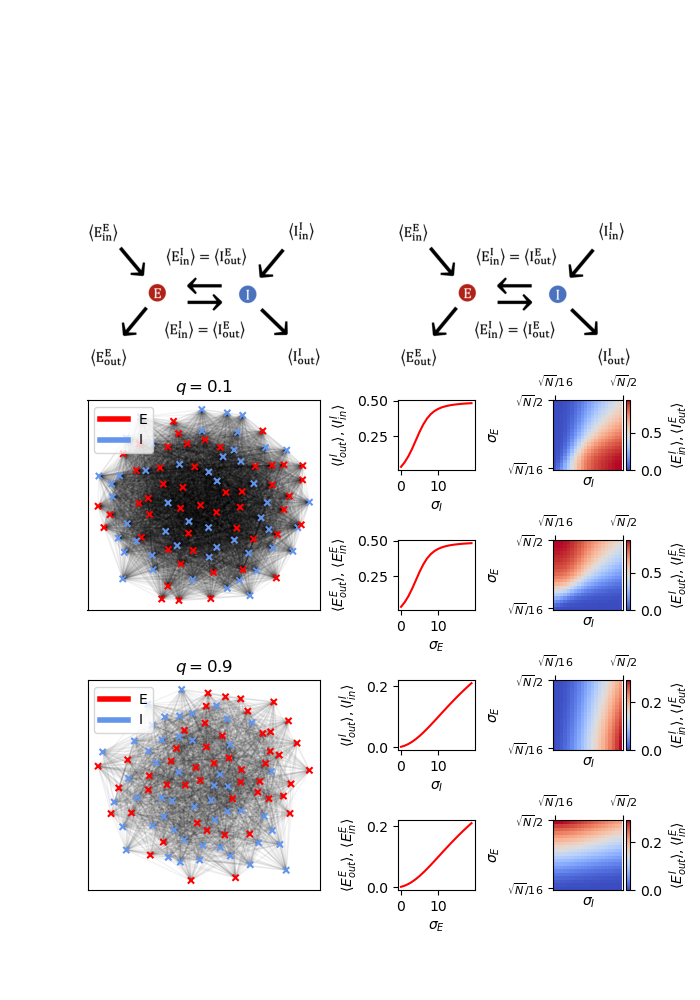
\includegraphics[width=175mm]{fig_9}
\caption{\textbf{Shared connections in a homogeneous Gaussian network} (A,B,C) The average number of shared incoming or outgoing connections $\langle S_{ij}\rangle /N$ as a function of distance between two neurons $|\Delta r_{ij}|$ for three different values of the reach parameter $\sigma$.}
\end{figure}

\clearpage



\subsection{Excitatory-inhibitory Gaussian networks}

Thus far we have considered only the case where the spatial connectivity kernel is the same for every neuron. However, the integrative properties of neurons depend strongly on the number, proportions and distribution of excitatory and inhibitory synaptic inputs they receive (Megias 2001). Also, the role excitatory-inhibitory balance in network dynamics has been a subject of recent debate. Indeed, balanced recurrent excitation and inhibition capture the irregular and asynchronous spiking activity with weak correlations reported in cortex. The spatial extent of excitation relative to inhibition has been shown to have a strong impact on network dynamics. In particular, when the spatial extent of excitation is sufficiently smaller than inhibition, the balanced fixed point loses stability (Rosenbaum 2014). 

To account for excitatory and inhibitory cell types within this framework, we must differentiate $\langle N_{ij}\rangle$ for excitatory and inhibitory neurons and solving for both the mean in-degree and out-degree separately. Thus we have the quantities $\langle E_{E}^{\mathrm{out}} \rangle,\langle E_{I}^{\mathrm{out}} \rangle,\langle E_{I}^{\mathrm{in}} \rangle$ and $\langle I_{E}^{\mathrm{out}} \rangle,\langle I_{I}^{\mathrm{out}} \rangle,\langle I_{E}^{\mathrm{in}} \rangle$. Under the assumption that excitatory and inhibitory neurons are distributed uniformly  in two-dimensional space, we have that $\langle E_{I}^{\mathrm{out}} \rangle = \langle I_{E}^{\mathrm{in}} \rangle$ and $\langle E_{I}^{\mathrm{in}} \rangle = \langle I_{E}^{\mathrm{out}}\rangle$. For brevity, we drop the superscripts and compute the above averages according the general prescription provided by (3.3). The result of these numerical calculations allow us to observe that, for $\Gamma_{0} = 0.2$, the fraction of the target population saturated by excitatory or inhibitory outputs increases monotonically with $\sigma_{E}$ and $\sigma_{I}$  (Fig 3.4 b,d). The parameter maps provided in (Fig 3.4 b,d) are a starting point for our later discussions of newtork dynamics. 


\clearpage
\begin{figure}[t!]
\centering
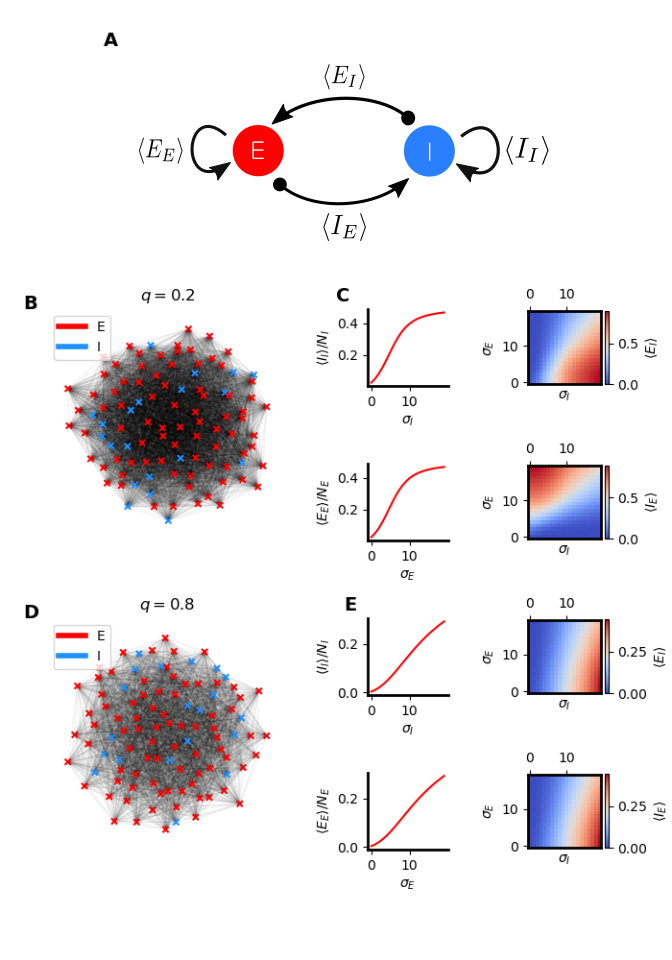
\includegraphics[width=165mm]{fig_10}
\caption{\textbf{Average degree in an excitatory-inhibitory network} (A) Schematic illustrating the notation used for excitatory-excitatory, excitatory-inhibitory, inhibitory-excitatory, and inhibitory-inhibitory synapses. (B) An example dense excitatory-inihbitory network ($\Gamma_{0}=0.2$) and $p_{E} = 0.8$. (C) Average number of synapses in the dense network normalized to the target population size as a function of parameters $\sigma_{E}$ and $\sigma_{I}$. (D) An example sparse excitatory-inihbitory network ($\Gamma_{0}=0.8$) and $p_{E} = 0.8$. (E) Average number of synapses in the sparse network normalized to the target population size as a function of parameters $\sigma_{E}$ and $\sigma_{I}$.}
\end{figure}

\chapter{Mean-field theory for cortical dynamics}

\section{Introduction}

Mean-field techniques are a common approach utilized in statistical mechanics, being first introduced in the description of phase transitions. More generally, a mean-field theory approximates the behavior of single units in many-body interacting systems with a large number of degrees of freedom. In the context of neuroscience, we may wish to estimate the synaptic current $I_{j}$ through the membrane of a neuron $j$ based on the average firing rate of the population and known features of the synaptic connectivity. The mathematical relationship between synaptic currents and firing rates is often called the \emph{transfer-function} of a neuron - a quantitative relationship that proves useful in probing neuron response properties when synaptic currents are known. For example, when a feedforward population is clamped to spike trains with well-defined statistics. Furthermore, it has been hypothesized that the temporal irregularity of spiking activity of cortical neurons \emph{in-vivo} is due to a balance of excitatory and inhibitory currents into the cortical cells (Vreeswijk, 1998). Indeed, the interaction of balanced excitatory and inhibitory synaptic currents with the intrinsic noise of neurons has strong implications for the coding scheme and metabolic efficiency in cortex (Sengupta, 2013). 

In practice, the spatially-dependent connectivity models defined in the previous chapter present a fairly large parameter space determining network dynamics. As an alternative to exploring that parameter space exhaustively, we make the appropriate simplifications in order to make predictions of network dynamics analytically. The regime in which excitatatory and inhibitory currents are balanced is a natural starting point for our investigation.

\section{Mean-field equations for population firing rates}

The total synaptic current into a neuron $i$ can be decomposed according to 

\begin{align}
I_{i}^{\alpha}(t) &= I_{\mathrm{ext}}^{\alpha}(t) + I_{\mathrm{rec}}^{\alpha}(t)\\
&= I_{\mathrm{ext}}^{\alpha}(t) + \sum_{\beta}\sum_{j} \frac{J_{ij}^{\alpha\beta}}{\sqrt{N}}(\phi * z^{\beta}_{j}(t))
\end{align}

For the sake of generality, the term $\phi * z(t)$ represents the convolution of the spike variable $z(t) = \Theta(v(t) - \theta)$ with a kernel $\phi$, determining the shape of the post-synaptic current in response to a spike. In the mean-field approximation we replace the currents in (3.2) by averaging over $t$ and indices of the summation $j$ and $k$. For a fully-connected network, we have

\begin{align}
\langle I_{i}^{\alpha}(t)\rangle &= \langle I_{\mathrm{ext}}^{\alpha}(t)\rangle + \sum_{\beta}\sum_{j} \frac{J_{ij}^{\alpha\beta}}{\sqrt{N}}\langle z_{j}^{\beta}(t)\rangle_{t,j}\\
&= \langle I_{\mathrm{ext}}^{\alpha}(t)\rangle + \sqrt{N}\sum_{\beta}J_{ij}^{\alpha\beta} r_{\beta}
\end{align}

If the network is not fully-connected and instead has spatial properties as presented in the previous chapter, (3.4) becomes

\begin{align}
\langle I_{i}^{\alpha}(t)\rangle &= \langle I_{\mathrm{ext}}^{\alpha}(t)\rangle + \sqrt{N}\sum_{\beta}J_{ij}^{\alpha\beta}p_{\alpha\beta}r_{\beta}
\end{align}

where we have used the identitiy $p_{\alpha\beta} = \tilde{p}_{\alpha\beta}p_{\alpha}$ with $\tilde{p}_{\alpha\beta}$ being the probability of a synapse of a neuron $\alpha$ onto type $\beta$ and $p_{\alpha}$ the probability of a neuron being of type $\alpha$. Writing (3.5) explicitly for an excitatory or inhibitory neuron $k$ gives

\begin{align}
\langle I_{k}^{e}(t)\rangle &= \langle I_{\mathrm{ext}}^{e}(t)\rangle + \sqrt{N}\left(J_{ee}p_{ee}r_{e} + J_{ie}p_{ie}r_{i}\right)\\
\langle I_{k}^{i}(t)\rangle &= \langle I_{\mathrm{ext}}^{i}(t)\rangle + \sqrt{N}\left(J_{ii}p_{ii}r_{i} + J_{ei}p_{ei}r_{e}\right)
\end{align}


Preventing blow-up of the synaptic currents requires that the sum in (3.5) scales as $\mathcal{O}\left(1/\sqrt{N}\right)$ s.t. as $N\rightarrow \infty$ 

\begin{align}
\underset{N\rightarrow \infty}{\mathrm{lim}}\langle I_{k}^{e}(t)\rangle &= \langle I_{\mathrm{ext}}^{e}(t)\rangle + J_{ee}p_{ee}r_{e} + J_{ie}p_{ie}r_{i}\\
\underset{N\rightarrow \infty}{\mathrm{lim}}\langle I_{k}^{i}(t)\rangle &= \langle I_{\mathrm{ext}}^{i}(t)\rangle + J_{ei}p_{ei}r_{e} + J_{ii}p_{ii}r_{i}
\end{align}

which gives

\begin{align}
r_{e} = \frac{\langle I_{\mathrm{ext}}^{e}\rangle J_{ii}p_{ii} - \langle I_{\mathrm{ext}}^{i}\rangle J_{ei}p_{ei}}{J_{ei}J_{ie}p_{ei}p_{ie} - J_{ee}J_{ii}p_{ee}p_{ii}}
\end{align}

\begin{align}
r_{i} = \frac{\langle I_{\mathrm{ext}}^{e}\rangle J_{ei}p_{ei} - \langle I_{\mathrm{ext}}^{i}\rangle J_{ee}p_{ee}}{J_{ei}J_{ie}p_{ei}p_{ie} - J_{ee}J_{ii}p_{ee}p_{ii}}
\end{align}


\section{Finite-size effects in numerical simulations}


\chapter{Synaptic plasticity in inferior temporal cortex}

Complex systems are ubiquitous in nature yet our scientific efforts have thus far only begun to gain traction on their governing principles. Many of the most intriguing complex systems in nature exihibit behaviors that simply cannot be explained by any of the components in isolation but rather arise from their complex interactions, bringing emergent phenomena into the focus of modern science. Such systems may be of physical, economic, or biological in nature, but all are thought to exihibit emergent properties under the appropriate conditions, suggesting broad relevance for the study of complex systems. 

To put complexity into perspective, consider the states of an interacting system of $N$ binary variables denoted $\{z_{i}\}_{i=1}^{N}$ which might be physically realized as an ensemble of spins in a ferromagnet. Even for extremely small cases such as $N=100$ the system can take on $2^{100} = 1.26\times 10^{30}$ different configurations and by $N=300$ the number of configurations exceed our best estimates for the number of atoms in the known universe. These unimaginabily large numbers simultaneously suggest that we cannot even hope to estimate a probability distribution over the phase space of the system, even with the most cutting edge experimental apparatus. The human cerebral cortex parallels this complexity, but maintains an order evident in the stability of our sensory percepts, in spite of its construction from over 16 billion noisy nerve cells. 

Neurons in cortex connect when afferent nerve fibers of a presynaptic cell meet a small patch of the dendritic tree or soma of a post-synaptic, forming the synapse. The complexity of neural networks arises from the complexity of these communication channels. It is a great challenge to understand how the complex connectivity patterns in cortex give rise to stable functions including the formation and retrieval of memories. In his famous neurophysiological postulate, Donald Hebb first proposed a cellular mechanism for the self-organization of networks of neurons [1]. Hebb suggested that repeated stimulation of specific receptors of sensory signals would lead slowly to the formation of a \emph{cell assembly} and these structural changes would constitute a representation or imprint of an internally or externally generated sensation e.g., an image or idea. This process, referred to as Hebbian learning, is argued to be driven by the temporal order of action potentials where the synaptic efficacy of the connection between neurons increases when a presynaptic neuron fires an action potential before a postsynaptic neuron.

Synaptic plasticity refers to the activity-dependent modification of the strength or efficacy of synaptic transmission at preexisting synapses, and has been proposed to play a central role in the incorporation of transient experiences into persistent memory traces. The efficacy of an excitatory synapse can be either potentiated or depressed by a variety of mechanisms which occur over a wide range of time scales: from milliseconds to hours to days. Short-term synaptic plasticity (STP) is thought to play an important role in information processing in the brain. Its duration allows STP to modify the response of cortical circuits to stimuli and potentially provide a richer set of response properties without permanently altering the circuit architecture. One of several mechanisms thought to underly STP can be seen by the repeated stimulation of a presynaptic cell causing a transient accumulation of calcium in the presynaptic terminal (Mongillo et al. 2008). Calcium generally thought to elevate the probability of neurotransmitter release due to its proposed interaction with the biochemical machinery involved in synaptic vesicle excytosis. Other short term changes in synaptic efficacy can occur such as the facilitation or depression based upon the temporal characteristics of the stimulus. In paired-pulse experiments, a pair of stimuli is delivered a sub-20ms interval shows depression of the efficacy of the second stimulus (Zucker and Regehr, 2002). This phenomenon is hypothesized to arise from inactivation of voltage-dependent sodium and/or calcium channels or depletion of the release ready pool of synaptic vesicles at the presynaptic terminal [1]. Synaptic efficacy can be lowered by the release of biochemical modulators which can interact with the synaptic machinery to inhibit the release of neurotransmitter into the synaptic cleft. In addition, receptors at the presynaptic terminal which play a role in the secretion of neurotransmitter are sensitive to the presence of presynaptic neurmodulators. Therefore, these neuromodulators can also play a role in facilitation or depression in STP.

It is widely believed that neural circuits also possess the mechanisms for long term changes in synaptic strength formally referred to as long term potentiation (LTP) and long term depression (LTD). The brain encodes internally and externally generated stimuli as spatiotemporal patterns of action potentials and long-term modifications to such patterns via changes in synaptic transmission provide a feasible mechanism for the storage of information. In other words, changes in synaptic weights alter the spatiotemporal response of population of neurons to stimuli and therefore provide a method for long term memory formation. Since its original introduction by Cajal, this idea has been rigorously tested, for example in the CA1 region of the hippocampus (Whitlock et al. 2006). LTP and LTD have been extensively studied in the CA1 region of the hippocampus due to compelling evidence that it is a brain region that is central to learning and memory. Indeed, the cellular and biochemical mechanisms underlying these phenomena have been well-characterized. 



\begin{appendices}
\chapter{The Kramers-Moyal expansion}

Given many instantiations of a stochastic variable $V$, we can construct a normalize histogram over all observations as a function of time $P(V,t)$. However, in order to systematically explore the relationship between the parameterization of the process and $P(V,t)$ we require an expression for $\dot{P}(V,t)$. If we make a fundamental assumption that the evolution of $P(V,t)$ follows a Markov process i.e. its evolution has the memoryless property, then we can write

\begin{equation}
P(V', t) = \int T(V', t | V, t-\tau)P(V, t-\tau)dV
\end{equation} 

which is known at the Chapman-Kolmogorov equation. The factor $T(V', t | V, t-\tau)$ is known as the \emph{transition operator} in a Markov process and determines the evolution of $P(V,t)$ in time. We proceed by writing $T(V', t | V, t-\tau)$ in a form referred to as the Kramers-Moyal expansion

\begin{align*}
T(V', t | V, t-\tau) &= \int \delta(u-V')T(u, t | V, t-\tau)du\\
&= \int \delta(V+u-V'-V)T(u, t | V, t-\tau)du\\
\end{align*} 

If we use the Taylor expansion of the $\delta$-function 

\begin{equation*}
\delta(V+u-V'-V) = \sum_{n=0}^{\infty} \frac{(u-V)^{n}}{n!}\left(-\frac{\partial}{\partial V}\right)^{n}\delta(V-V')
\end{equation*}

Inserting this into the result from above, pulling out terms independent of $u$ and swapping the order of the sum and integration gives

\begin{align}
T(V', t | V, t-\tau) &= \sum_{n=0}^{\infty} \frac{1}{n!}\left(-\frac{\partial}{\partial V}\right)^{n}\delta(V-V')\int(u-V)^{n}T(u, t | V, t-\tau)du\\
&= \sum_{n=0}^{\infty} \frac{1}{n!}\left(-\frac{\partial}{\partial V}\right)^{n}\delta(V-V')M_{n}(V,t)
\end{align} 

noticing that $M_{n}(V,t) = \int(u-V)^{n}T(u, t | V, t-\tau)du$ is just the $n$th moment of the transition operator $T$. Plugging (2.6) back in to (2.4) gives 

\begin{align}
P(V, t) &= \int \left(1 + \sum_{n=1}^{\infty} \frac{1}{n!}\left(-\frac{\partial}{\partial V}\right)^{n} M_{n}(V,t)\right)\delta(V-V')P(V, t-\tau)dV\\
&= P(V', t-\tau) + \sum_{n=1}^{\infty} \frac{1}{n!}\left(-\frac{\partial}{\partial V}\right)^{n} \left[M_{n}(V,t)P(V,t)\right]
\end{align} 

Approximating the derivative as a finite difference and taking the limit $\tau\rightarrow 0$ gives

\begin{align}
\dot{P}(V,t)  &= \underset{\tau\rightarrow 0}{\mathrm{lim}}\left(\frac{P(V, t)-P(V, t-\tau)}{\tau}\right)\\
&= \sum_{n=1}^{\infty} \frac{1}{n!}\left(-\frac{\partial}{\partial V}\right)^{n} \left[M_{n}(V,t)P(V,t)\right]
\end{align} 

which is formally known as the Kramers-Moyal (KM) expansion. The Fokker-Planck equation is a special case of (2.10) where we neglect terms $n>2$ in the \emph{diffusion approximation}.
\end{appendices}

% Format a LaTeX bibliography
\makebibliography

[1] D.O. Hebb \textit{The organization of behavior: A neurophysiological theory}. John Wiley and Sons. 1949.

% Figures and tables, if you decide to leave them to the end
%\input{figure}
%\input{table}

\end{document}


